\usetikzlibrary{arrows.meta}
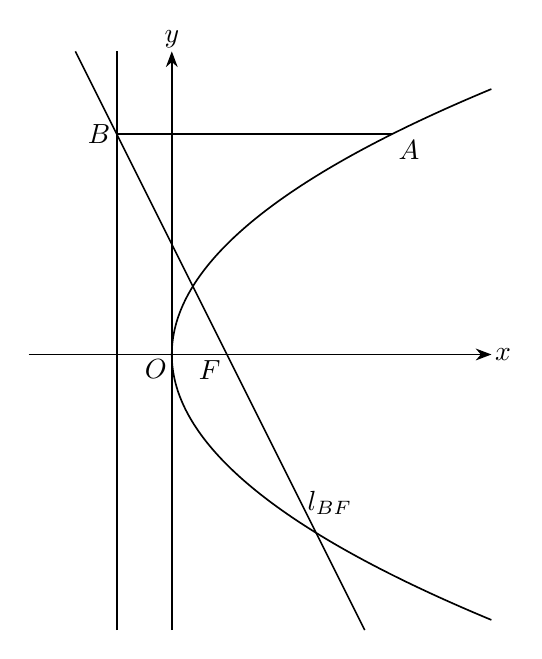
\begin{tikzpicture}[x=0.7cm,y=0.7cm,line width=.6pt,font=\normalsize,>=Stealth]
\coordinate (O) at (0,0);
\coordinate (F) at (1,0);
\coordinate (A) at (4,4);
\coordinate (B) at (-1,4);
\draw[->] (-2.6,0)--(5.8,0) node[right,inner sep=1pt] {$x$};
\draw[->] (0,-5.0)--(0,5.5) node[above,inner sep=1pt] {$y$};
\draw (-1,-5.0)--(-1,5.5);
\draw[domain=-4.816:4.816,samples=160] plot ({\x*\x/4},{\x});
\draw (B)--(A);
\draw (-1.75,5.5)--(3.5,-5.0);
\node[below left,inner sep=1.5pt] at (O) {$O$};
\node[below left,inner sep=2pt] at (F) {$F$};
\node[below right,inner sep=2pt] at (A) {$A$};
\node[left,inner sep=2pt] at (B) {$B$};
\node[right=2pt,inner sep=0pt] at (2.35,-2.7) {$l_{BF}$};
\end{tikzpicture}
